\documentclass[a4paper,12pt]{article}

\usepackage[utf8]{inputenc}
\usepackage[russian]{babel}
\usepackage[left=17mm, right=15mm, top=20mm, bottom=20mm]{geometry}
\usepackage{pscyr}
\usepackage{graphicx}
    \graphicspath{ {.} }
\usepackage{hyperref}
    \hypersetup{
        colorlinks=true,
        linkcolor=blue,
        filecolor=magenta,      
        urlcolor=cyan,
    }


\begin{document}
    \begin{center}
        \thispagestyle{empty}
        \large САНКТ-ПЕТЕРБУРГСКИЙ ГОСУДАРСТВЕННЫЙ ПОЛИТЕХНИЧЕСКИЙ УНИВЕРСИТЕТ им. ПЕТРА ВЕЛИКОГО

        Институт компьютерных наук и технологий

        Высшая школа искусственного интеллекта
        \vspace{9cm}

        Отчет по курсовой работе

        \huge Игра в дурака
    \end{center}
    \vspace{6cm}
    \begin{flushright}
        \large
        Работу выполнил:

        Алехичев~А.\,В.

        группа~3530201/10001
        \vspace{2mm}

        Проверил:

        Курочкин~Л.\,М.
    \end{flushright}
    \begin{center}
        \large Санкт-Петербург - 2022\,г.
    \end{center}

    \newpage

    \tableofcontents

    \newpage

    \section{Постановка задачи}
        \begin{enumerate}
            \item Разработать алгоритм, который может играть в дурака в качестве игрока по заданным правилам
            \begin{itemize}
                \item Правила находятся в \texttt{/doc/rules.jpg} или по \href{http://13633-oop.mooo.com/files/durak.docx}{ссылке}
            \end{itemize}
            \item Реализовать алгоритм на языке C++
            \begin{itemize}
                \item Для работы с~колодой использовать статическую библиотеку \texttt{/dealer.lib}.
                \item Сопроводительные файлы к лабораторной и библиотека \textsf{dealer} доступны по~ссылкам: \href{http://13633-oop.mooo.com/files/dealer_vs2019.zip}{WIN32} или \href{http://13633-oop.mooo.com/files/dealer_x86_64.zip}{Linux64}
            \end{itemize}
            \item Подготовить отчёт по~работе, соответствующий требованиям
            \begin{itemize}
                \item Требования находятся в~\texttt{/doc/kr\_req.docx} или по~\href{http://13633-oop.mooo.com/files/kr_req.docx}{ссылке}
                \item Задокументировать разработанный алгоритм и написанный по~нему код
            \end{itemize}
        \end{enumerate}

    \section{Описание исходных данных задачи}

    \subsection{Алгоритм игры в дурака}
        Данный алгоритм определяет возможные ходы для двух игроков, то как они взаимодействуют и различные состояния игры.
        Алгоритм представлен в~виде блок-схемы, а~также в~файле \texttt{/main.cpp},
        распространяющемся в~одном zip-архиве с~библиотекой dealer.
        Блок-схему можно посмотреть в~\hyperlink{rulesimg}{приложении 1}

    \subsection{Статическая библиотека \textsf{dealer}}
        Дана статическая библиотека \textsf{dealer}.
        Эта библиотека отвечает за контроль колоды и стола.
        К~этому относится: хранение, перетасовка колоды, получение информации о~колоде, взятие карты из~колоды.
        А~также получение информации о~козырной масти и столе.
    
    \section{Определение терминов}
        \subsection{Ранг карты}
            \begin{itemize}
                \item[] Свойство карты.
                \item[] Ранг карты выражается с помощью целого числа --- типа~\texttt{int}.
                \item[] С помощью метода \texttt{Dealer::RankIndex} можно узнать ранг карты.
                \item[] Ранг обычной карты можно использовать как индекс в массиве \texttt{ranks}, чтобы получить имя ранга.
                \item[] Ранг особой карты используется как обозначение состояния особых карт.
                \item[] Данные состояния --- <<Пас>> и <<Без карты>> выражаются числами 300 и 400 соответственно.\\
                        Эти числа указаны в коде как \texttt{PAS} и \texttt{NOCARD}.
                \item[] Ранги обычной карты можно сравнить.
                        Величина ранга увеличивается в порядке:\\
                        \texttt{2 < 3 < 4 < 5 < 6 < 7 < 8 < 9 < 10 < Jack < Queen < King < Ace}.
            \end{itemize}

        \subsection{Масть карты}
            \begin{itemize}
                \item[] Свойство карты.
                \item[] Масть карты выражается с помощью целого числа --- типа~\texttt{int}.
                \item[] С помощью метода \texttt{Dealer::SuitIndex} можно узнать масть карты.
                \item[] Масть обычной карты можно использовать как индекс в массиве \texttt{suits}, чтобы получить имя масти.
                \item[] Масть обычной карты можно использовать как индекс в массиве \texttt{suitsSymb}, чтобы получить символ масти.
                \item[] Масть может быть \textit{козырной}.
                        Масть считается козырной, если совпадает\\с мастью, выбранной дилером до начала игры.\\
                        Эту масть можно узнать с помощью\\метода \texttt{Dealer::GetTrump}.
            \end{itemize}

        \subsection{Карта}
            \begin{itemize}
                \item[] Обычная карта имеет одну из четырёх мастей и один из тринадцати рангов.
                \item[] Особая карта может находиться в одном из двух дополнительных особых состояний: <<Пас>> или <<Без карты>>.
                        В таком случае, её ранг будет равен \texttt{PAS} или \texttt{NOCARD} соответственно.
                \item[] Обычная карта может быть \textit{козырной}.
                        Карта считается козырной, если у неё козырная масть.
                \hypertarget{hit_rule}{
                \item[] Карта может быть <<атакующей>> или <<защищающей>>.
                        Карта, которой играет игрок с инициативой, называется атакующей.
                        Карта, которой его оппонент может согласно правилам может
                        побить атакующую карту, называется защищающая.
                \item[] <<Атакующую>> карту можно побить <<защищающей>>. Это возможно в одном из двух случаев:
                }
                \begin{itemize} 
                    \item Если карты имеют одинаковую масть, то атакующую карту можно побить защищающей в случае если у первой ранг меньше, чем у второй.
                    \item Если карты имеют разную масть, то атакующую карту любого ранга можно побить козырной защищающей картой любого ранга.
                \end{itemize}
            \end{itemize}

        \subsection{Колода}
            \begin{itemize}
                \item[] Последовательный набор уникальных не особых карт.
                \item[] В начале игры колода из каждой возможной обычной карты перемешивается случайным образом.
                        Таким образом до начала игры в колоде 52 карты.\\
                        За перемешивание колоды отвечает метод \texttt{Dealer::ShuffleDec}
                \item[] Дилер может доставать из колоды карты.
            \end{itemize}

        \subsection{Ход}
            \begin{itemize}
                \item[] Ход это последовательность действий игроков,
                        начинающаяся началом игры или концом другого хода,
                        и заканчивающаяся тем, что игрок без инициативы успешно
                        защитился от атакующих карт или не смог защититься.
                \item[] За ход игрок с инициативой может атаковать шестью картами, в согласии с правилами. 
            \end{itemize}

        \subsection{Стол}
            \begin{itemize}
                \item[] Стол это место, куда игроки разыгрывают карты в соответствии с правилами.
                \item[] На столе лежат карты. Стол имеет тип \texttt{Card*[6]}.
                \item[] За один ход игроки могут сыграть по 6 карт каждый.
            \end{itemize}

        \subsection{Дилер}
            \begin{itemize}
                \item[] Дилер отвечает за управление колодой и столом.
                \item[] Дилер в коде отображён как класс \texttt{Dealer}.
                \item[] Дилер достаёт карты из колоды и раздаёт игрокам в соответствии с правилами игры.\\
                        За это отвечает метод \texttt{Dealer::GetCard}.
                \item[] У дилера можно спросить козырную масть.\\
                        За это отвечает метод \texttt{Dealer::GetTrump}.
                \item[] У дилера можно спросить число вышедших из колоды карт.\\
                        За это отвечает метод \texttt{Dealer::getcurrentCard}
                \item[] У дилера можно получить указатель на стол.\\
                        За это отвечает метод \texttt{Dealer::GetheadTrick}.
                \item[] У дилера можно узнать номер текущей атакующей карты в ходе.\\
                        За это отвечает метод \texttt{Dealer::GetCurrentHeadTrik}.
                \item[] У дилера можно узнать можно ли сходить атакующей картой.\\
                        За это отвечает метод \texttt{Dealer::NextTrikEnable}.
                \item[] У дилера можно попросить особые карты ''пас'' и ''без карты''.\\
                        За это отвечают методы \texttt{Dealer::GetPas} и \texttt{Dealer::GetNocard}.
                \item[] У дилера можно узнать последнюю атакующую или защищающую карту.\\
                        За это отвечают методы \texttt{Dealer::GetLastCard} и \texttt{Dealer::GetLastDefendCard}
                \item[] Только с помощью дилера можно атаковать или защищаться картой.\\
                        За это отвечают методы \texttt{Dealer::Attack} и \texttt{Dealer::Defend}.
                \item[] Дилер проверяет карты на столе на корректность.\\
                        За это отвечает метод \texttt{Dealer::CheckHeadTrick}.
                \item[] После каждого хода дилер очищает стол от карт.\\
                        За это отвечает метод \texttt{Dealer::ClearTable}.
            \end{itemize}
            
        \subsection{Игрок}
            \begin{itemize}
                \item[] Игрок --- алгоритм или человек, принимающий не противоречащие правилам решения в игре.
                \item[] Один игрок играет лишь за одну сторону.
            \end{itemize}
    
    \section{Описание реализации}
        \subsection{Метод Player::YouTurn}
            



    \newpage
    \section{Приложения}
    \hypertarget{rulesimg}{\subsection{Блок-схема алгоритма игры в~дурака (\texttt{/main.cpp})}}
    \begin{figure}[h!]
        \center{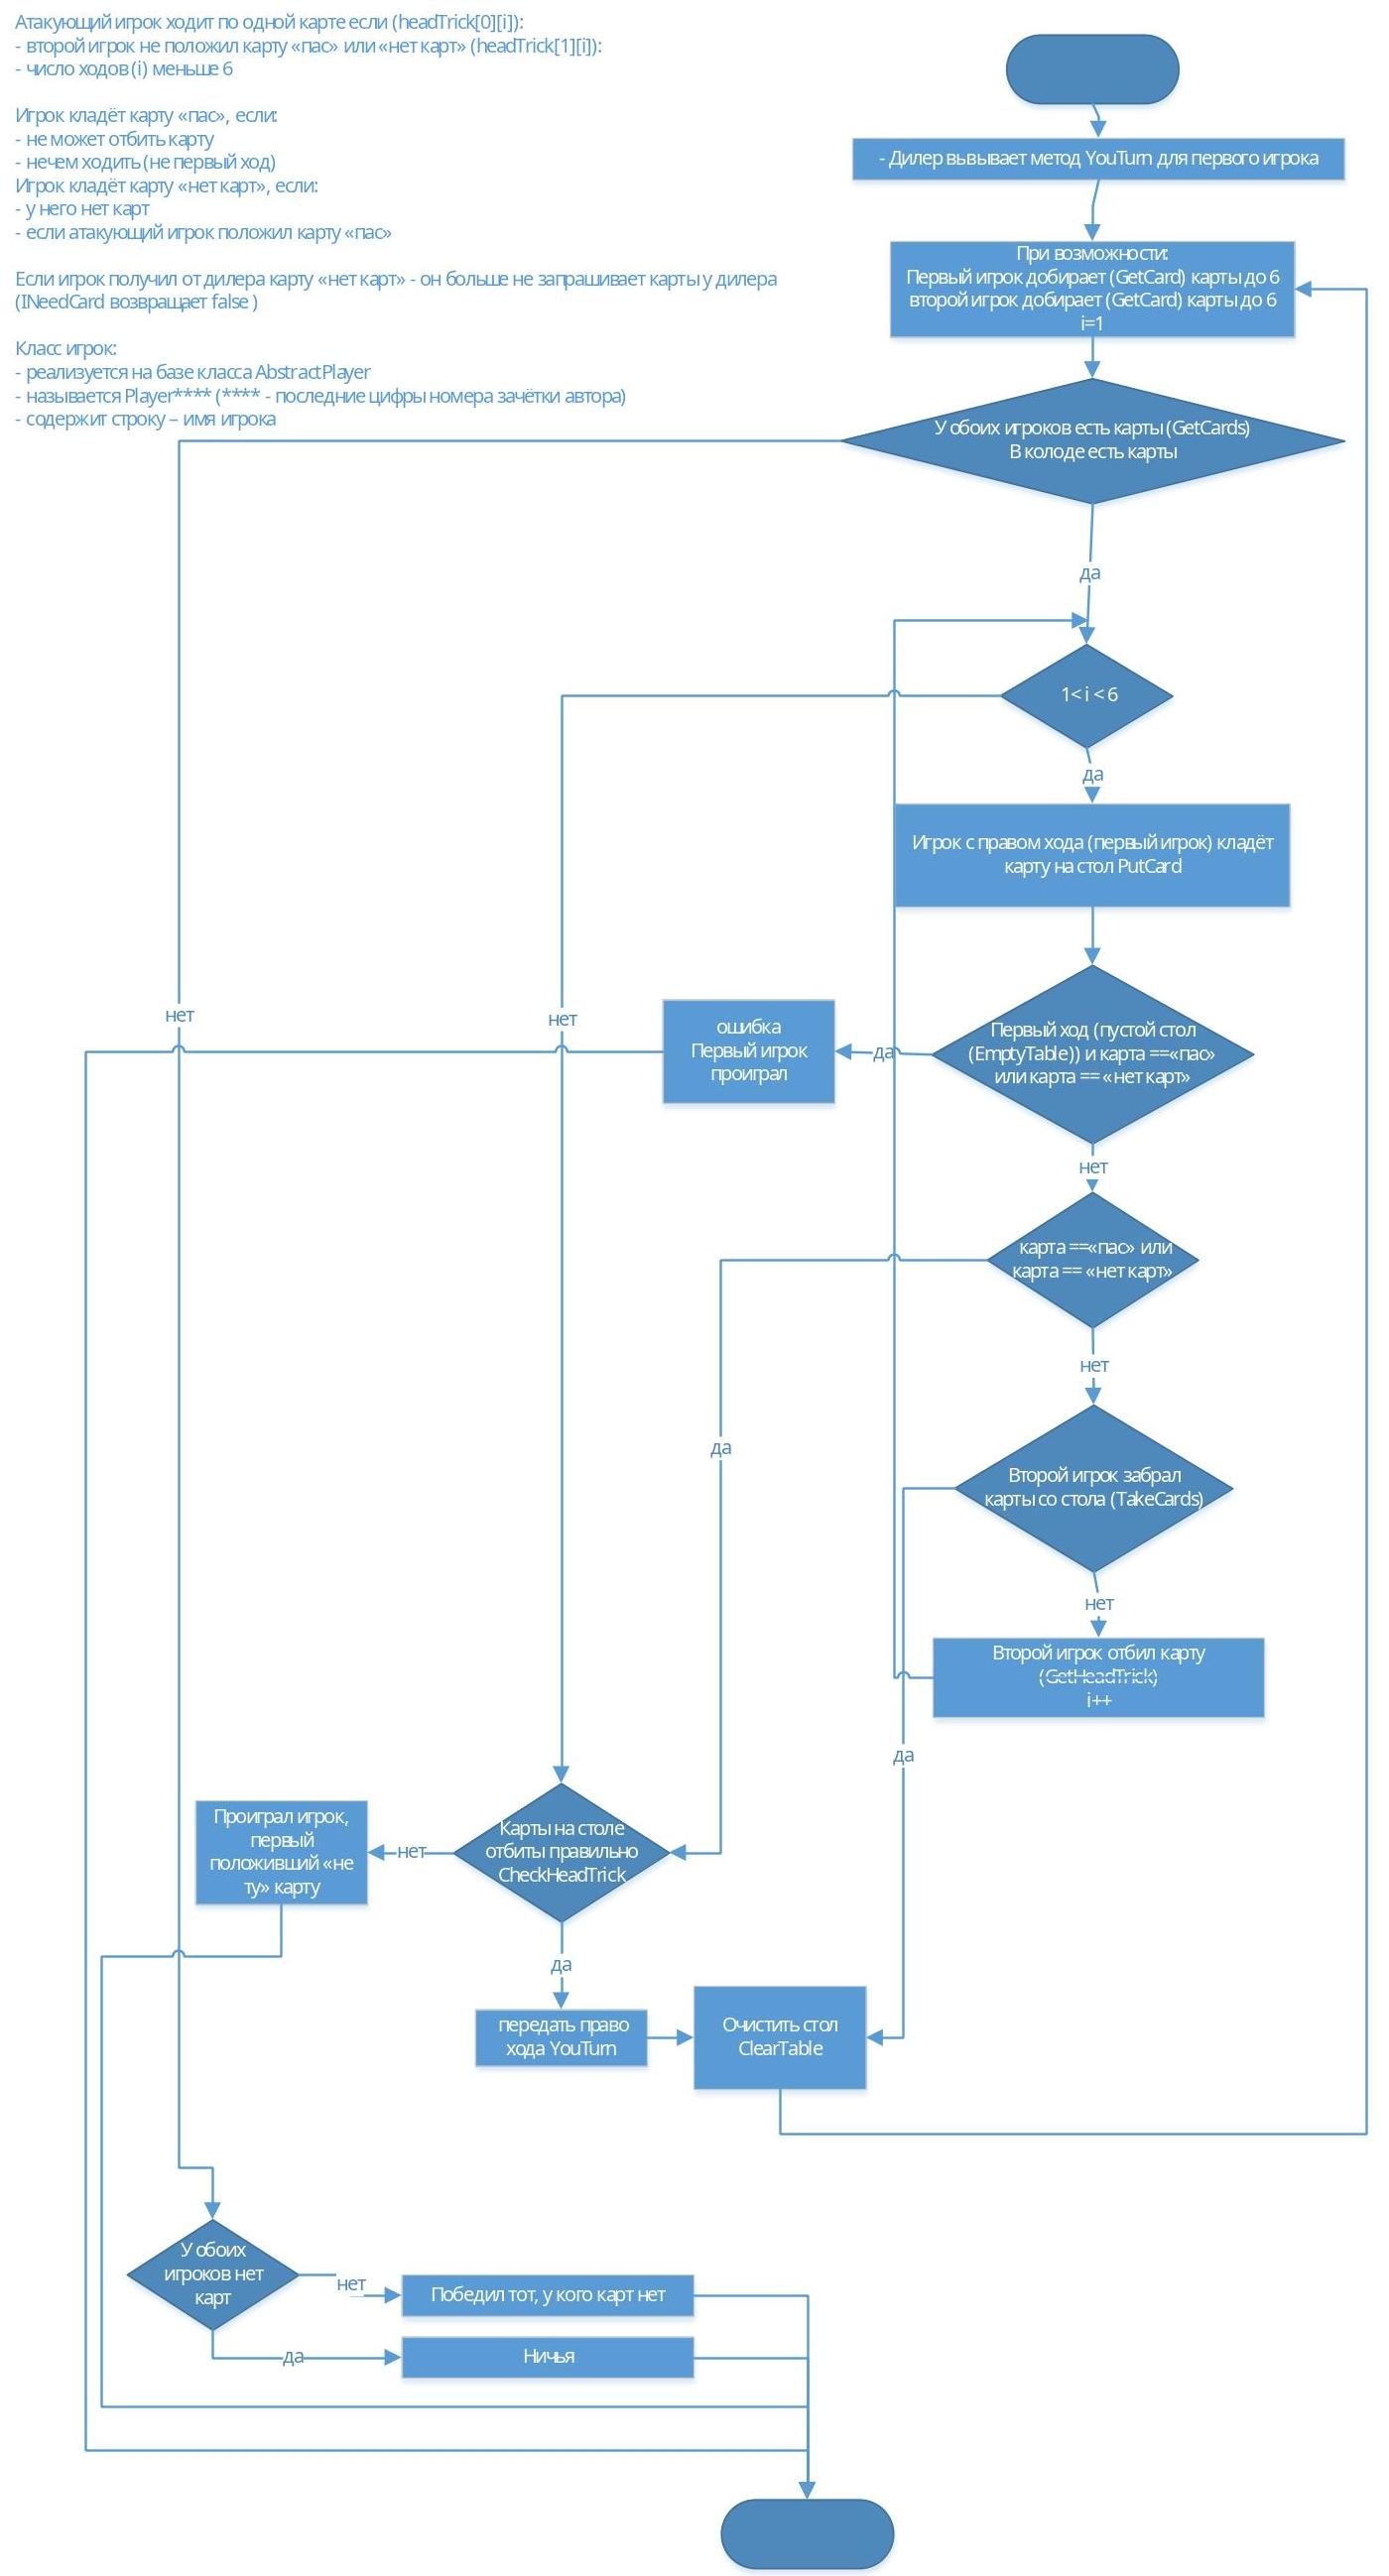
\includegraphics[height=0.9\textheight]{rules.jpg}}
    \end{figure}
    \newpage
    \subsection{Another}
    %\section{Литература}
    %\newpage
\end{document}
